\documentclass[]{article}
\voffset=-1.5cm
\oddsidemargin=0.0cm
\textwidth = 470pt
\usepackage[utf8]{inputenc}
\usepackage[english]{babel}
\usepackage{framed}

\usepackage{multicol}
\usepackage{amsmath}
\usepackage{amssymb}
\usepackage{enumerate}
\usepackage{multicol}




%opening
\title{Trees - Tutorial Sheet B}


\begin{document}
\begin{enumerate}
\item  \textbf{(Part A : Spanning Trees -  INSERT IMAGE) }\\
%\begin{figure}[h!]
%\centering
%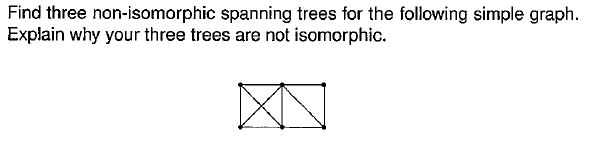
\includegraphics[width=1.11\linewidth]{TreesQuestion2012}
%\end{figure}

\begin{enumerate}[(i)]
\item How many edges are in the spanning tree $T$ ?
\item What is the sum of the degree sequence of $T$?
\item Write down all the possible degree sequences for the spanning tree $T$.
\end{enumerate}
\item 
Suppose a database, comprised of 30,000 internal nodes, is structured as a Binary Search Tree.

\begin{enumerate}[(i)]
\item What is the Key of the Root node?
\item What are the keys of the nodes at level 1?
\item For the nodes at level 1, how many subtrees are there?
\item State which nodes are in the substrees of the level 1 nodes?
\item How many nodes are the between the root (level 0) and level 4. 
(Hint: use a summation theorem mentioned in session 7
\item What is the maximum number of searchs in this database?
\end{enumerate}


\end{enumerate}

\end{document}